% Options for packages loaded elsewhere
\PassOptionsToPackage{unicode}{hyperref}
\PassOptionsToPackage{hyphens}{url}
%
\documentclass[
]{article}
\usepackage{amsmath,amssymb}
\usepackage{lmodern}
\usepackage{iftex}
\ifPDFTeX
  \usepackage[T1]{fontenc}
  \usepackage[utf8]{inputenc}
  \usepackage{textcomp} % provide euro and other symbols
\else % if luatex or xetex
  \usepackage{unicode-math}
  \defaultfontfeatures{Scale=MatchLowercase}
  \defaultfontfeatures[\rmfamily]{Ligatures=TeX,Scale=1}
\fi
% Use upquote if available, for straight quotes in verbatim environments
\IfFileExists{upquote.sty}{\usepackage{upquote}}{}
\IfFileExists{microtype.sty}{% use microtype if available
  \usepackage[]{microtype}
  \UseMicrotypeSet[protrusion]{basicmath} % disable protrusion for tt fonts
}{}
\makeatletter
\@ifundefined{KOMAClassName}{% if non-KOMA class
  \IfFileExists{parskip.sty}{%
    \usepackage{parskip}
  }{% else
    \setlength{\parindent}{0pt}
    \setlength{\parskip}{6pt plus 2pt minus 1pt}}
}{% if KOMA class
  \KOMAoptions{parskip=half}}
\makeatother
\usepackage{xcolor}
\usepackage[margin=1in]{geometry}
\usepackage{graphicx}
\makeatletter
\def\maxwidth{\ifdim\Gin@nat@width>\linewidth\linewidth\else\Gin@nat@width\fi}
\def\maxheight{\ifdim\Gin@nat@height>\textheight\textheight\else\Gin@nat@height\fi}
\makeatother
% Scale images if necessary, so that they will not overflow the page
% margins by default, and it is still possible to overwrite the defaults
% using explicit options in \includegraphics[width, height, ...]{}
\setkeys{Gin}{width=\maxwidth,height=\maxheight,keepaspectratio}
% Set default figure placement to htbp
\makeatletter
\def\fps@figure{htbp}
\makeatother
\setlength{\emergencystretch}{3em} % prevent overfull lines
\providecommand{\tightlist}{%
  \setlength{\itemsep}{0pt}\setlength{\parskip}{0pt}}
\setcounter{secnumdepth}{-\maxdimen} % remove section numbering
\ifLuaTeX
  \usepackage{selnolig}  % disable illegal ligatures
\fi
\IfFileExists{bookmark.sty}{\usepackage{bookmark}}{\usepackage{hyperref}}
\IfFileExists{xurl.sty}{\usepackage{xurl}}{} % add URL line breaks if available
\urlstyle{same} % disable monospaced font for URLs
\hypersetup{
  pdftitle={Student performance analysis},
  pdfauthor={Olawal},
  hidelinks,
  pdfcreator={LaTeX via pandoc}}

\title{Student performance analysis}
\author{Olawal}
\date{2023-06-01}

\begin{document}
\maketitle

\hypertarget{table-of-contents}{%
\subsection{Table of contents}\label{table-of-contents}}

\hypertarget{introduction}{%
\subsubsection{1. Introduction}\label{introduction}}

\hypertarget{design}{%
\subsubsection{2. Design}\label{design}}

\hypertarget{implementation}{%
\subsubsection{3. Implementation}\label{implementation}}

\hypertarget{user-guide}{%
\subsubsection{4. User guide}\label{user-guide}}

\hypertarget{conclusion}{%
\subsubsection{5. Conclusion}\label{conclusion}}

\hypertarget{bibliography}{%
\subsubsection{6. Bibliography}\label{bibliography}}

\hypertarget{appendix}{%
\subsubsection{7. Appendix}\label{appendix}}

\newpage

\hypertarget{introduction-1}{%
\paragraph{Introduction}\label{introduction-1}}

Motivation

Higher education is critical to an individual's future success.
Predicting academic success becomes increasingly crucial as more kids
enter colleges and universities.Alyahyan and Düştegör (2020). As a
student, I have witnessed students struggle with low academic
achievement owing to a variety of causes, and by employing data
exploration techniques, I am able to uncover critical aspects that
influence a student's success. In this study, I hope to analyse three of
these publicly available datasets in order to better understand the
various factors that influence college students' academic achievement.
My study, I hope, will assist institutions in identifying students at
risk of poor performance and providing them with the assistance they
require to achieve academically. Furthermore, this initiative will
assist education policymakers in developing effective interventions to
increase overall student performance.

Questions we seek to address through this analysis are;

● What are the significant factors that affect the academic performance
of students?\\
● Are there any significant differences in academic performance between
students of different\\
ethnicities or races, and if so, what factors contribute to these
differences?\\
● How do these factors impact the academic performance of students?

\newpage

\hypertarget{implementation-1}{%
\paragraph{Implementation}\label{implementation-1}}

\hypertarget{tech-stack-used-in-developing-the-dashboard}{%
\subparagraph{Tech stack used in developing the
dashboard}\label{tech-stack-used-in-developing-the-dashboard}}

\begin{enumerate}
\def\labelenumi{\arabic{enumi}.}
\tightlist
\item
  R Shiny\\
\end{enumerate}

\begin{itemize}
\tightlist
\item
  Shiny is an R package that makes it easy to build interactive web apps
  straight from R. You can host standalone apps on a webpage or embed
  them in R Markdown documents or build dashboards.\\
  One of the advantages of using R Shiny is that its open source, as
  such we don't need licence to use it.
\end{itemize}

\begin{enumerate}
\def\labelenumi{\arabic{enumi}.}
\setcounter{enumi}{1}
\tightlist
\item
  Cascading Styling Sheet\\
\end{enumerate}

\begin{itemize}
\tightlist
\item
  Cascading Style Sheets is a style sheet language used for describing
  the presentation of a document written in a markup language such as
  HTML. CSS is a cornerstone technology of the World Wide Web, alongside
  HTML and JavaScript.
\end{itemize}

\hypertarget{packages-used-in-developing-the-dashboard}{%
\subparagraph{Packages used in developing the
dashboard:}\label{packages-used-in-developing-the-dashboard}}

\begin{itemize}
\tightlist
\item
  shiny

  \begin{itemize}
  \tightlist
  \item
    R package for creating web applications.\\
    For more, click \href{https://shiny.rstudio.com/tutorial/}{here}
  \end{itemize}
\item
  dplyr

  \begin{itemize}
  \tightlist
  \item
    dplyr is a grammar of data manipulation, providing a consistent set
    of verbs that help you solve the most common data manipulation
    challenges.\\
    For more, click
    \href{https://cran.r-project.org/web/packages/dplyr/vignettes/dplyr.html}{here}
  \end{itemize}
\item
  ggplot2

  \begin{itemize}
  \tightlist
  \item
    ggplot2 is a system for declaratively creating graphics, based on
    The Grammar of Graphics. You provide the data, tell ggplot2 how to
    map variables to aesthetics, what graphical primitives to use, and
    it takes care of the details.\\
    For more, click \href{https://ggplot2.tidyverse.org/}{here}
  \end{itemize}
\item
  plotly

  \begin{itemize}
  \tightlist
  \item
    Create interactive web graphics from `ggplot2' graphs and/or a
    custom interface to the (MIT-licensed) JavaScript library
    `plotly.js' inspired by the grammar of graphics.\\
    For more, click \href{https://plotly.com/r/getting-started/}{here}
  \end{itemize}
\item
  data.table

  \begin{itemize}
  \tightlist
  \item
    For data wrangling and manipulation.\\
    For more, click
    \href{https://cran.r-project.org/web/packages/data.table/vignettes/datatable-intro.html}{here}
  \end{itemize}
\item
  flexdashboard

  \begin{itemize}
  \tightlist
  \item
    The goal of flexdashboard is to make it easy to create interactive
    dashboards for R. Used the gauge function from this library to
    create gauge plot.
  \end{itemize}
\item
  shinythemes

  \begin{itemize}
  \tightlist
  \item
    Used to improve the overall appearance of shiny dashboards.
  \end{itemize}
\end{itemize}

\newpage

\hypertarget{challenges}{%
\subparagraph{Challenges}\label{challenges}}

R Shiny is not a native web language and this paused a challenge in
developing the user interface. To make the interface/theming appealing,
I used css to alter the user interface of the R Shiny dashboard.

\hypertarget{user-guide-1}{%
\paragraph{User guide}\label{user-guide-1}}

The dashboard has two sections:

\begin{itemize}
\tightlist
\item
  Header\\
\item
  Mainpanel
\end{itemize}

\hypertarget{header}{%
\subparagraph{Header}\label{header}}

This section of the dashboard has the title of the application which
basically is meant to give an idea of what dashboard is all about.


\includegraphics[width=5.20833in,height=0.52083in]{www/header.png}

\hypertarget{main-panel}{%
\subparagraph{Main panel}\label{main-panel}}

This is where we have the various graphs that give insights into the
data.

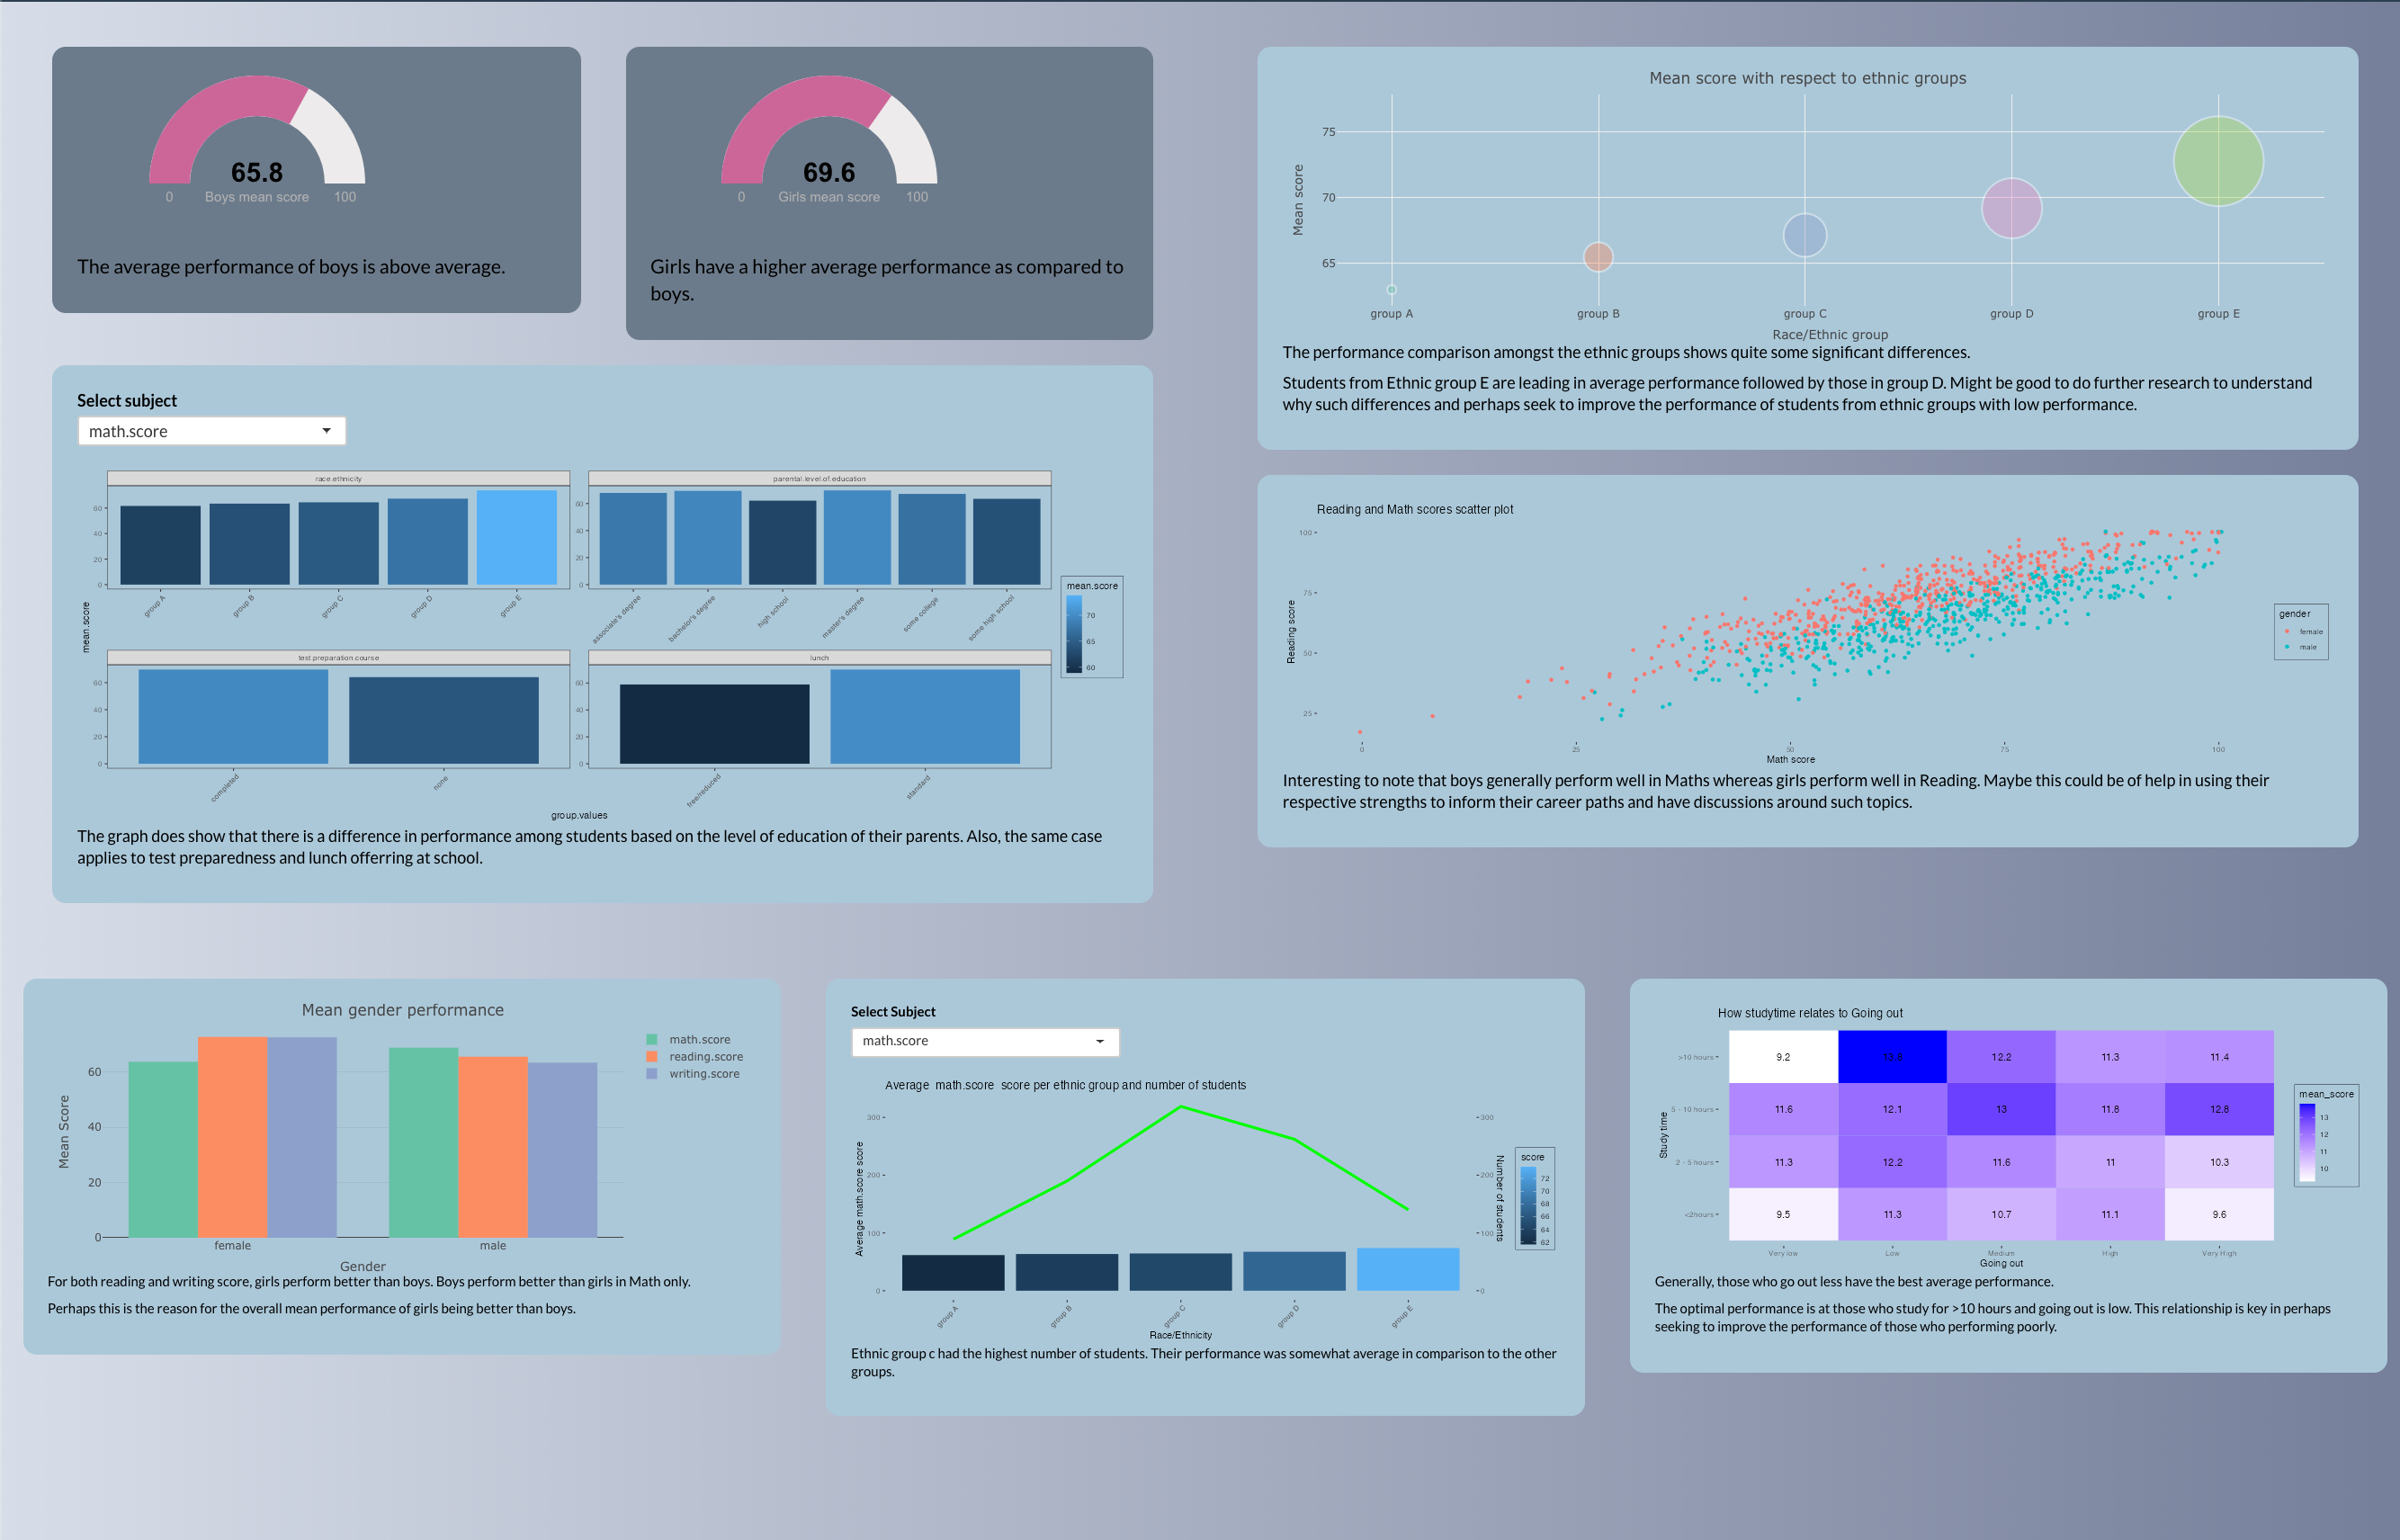
\includegraphics[width=5.20833in,height=2.08333in]{www/mainpanel.png}

\newpage

\hypertarget{gauge-plots}{%
\subparagraph{Gauge plots}\label{gauge-plots}}

This kind of graphs are ideal in cases where you have some sort of
target, like in this case the target score is 100. So the gauge is at
the mean score and it shows what's left against the target. Perfect fit
to show the average performance of boys and girls adrift the target
score.

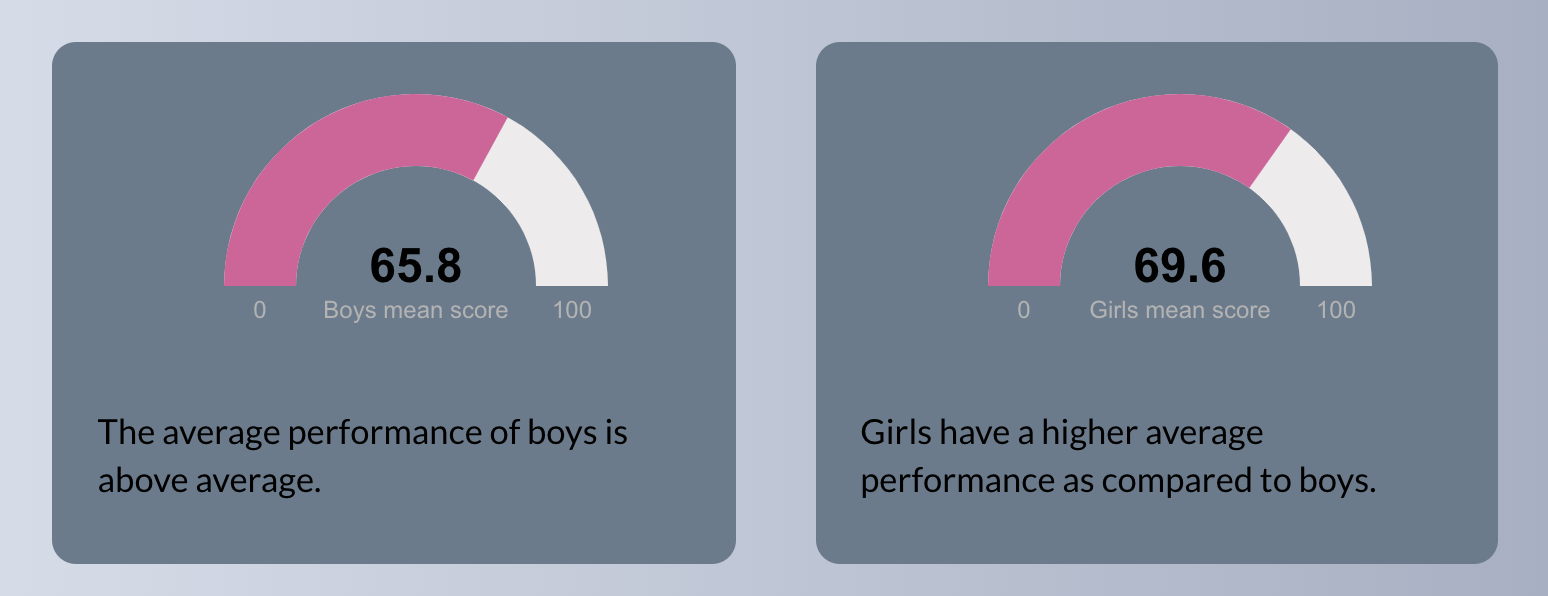
\includegraphics[width=5.20833in,height=2.08333in]{www/gauge.png}

\newpage

\hypertarget{bubble-plot}{%
\subparagraph{Bubble plot}\label{bubble-plot}}

This kind of plot is a good alternative to bar graphs. It fits well in
cases where you want to visualize categorical data with respect to
quantities. The size of the bubble corresponds to the numeric value for
a given item. In this case we see the average performance per ethnic
group. The plot brings out the comparisons well, note that the graph is
interactive, the user can hover on the graph to see average score and
the respective ethnic group.

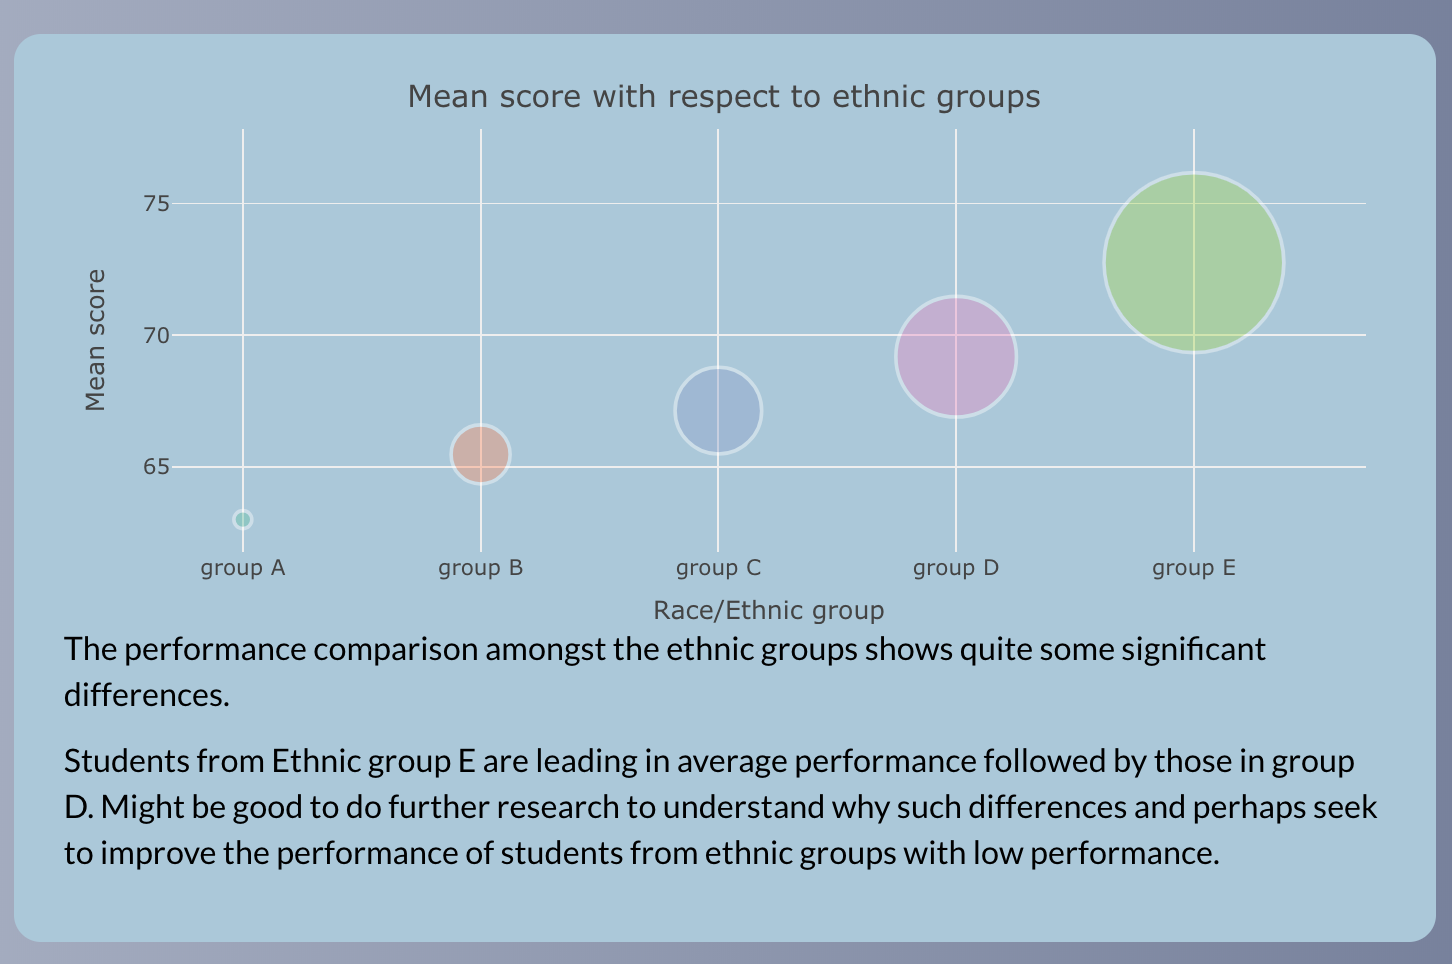
\includegraphics[width=5.20833in,height=2.08333in]{www/bubble.png}

\newpage

\hypertarget{combined-bar-graphs}{%
\subparagraph{Combined bar graphs}\label{combined-bar-graphs}}

Ggplot2 R graphing library has this amazing feature where you can have
multiple bar charts faceted on a group variable. This feature was used
to plot the average score for multiple variable; parents education
levels, lunch, test preparation and ethnic group. This graph is a good
way to combine multiple graphs into one instead of plotting them
separately.\\
Additionally, we have a dropdown menu that the use can use to select the
view per selected subject.\\
Also, the graph has a legend for guiding the user on the color used and
how it relates to the various score values.

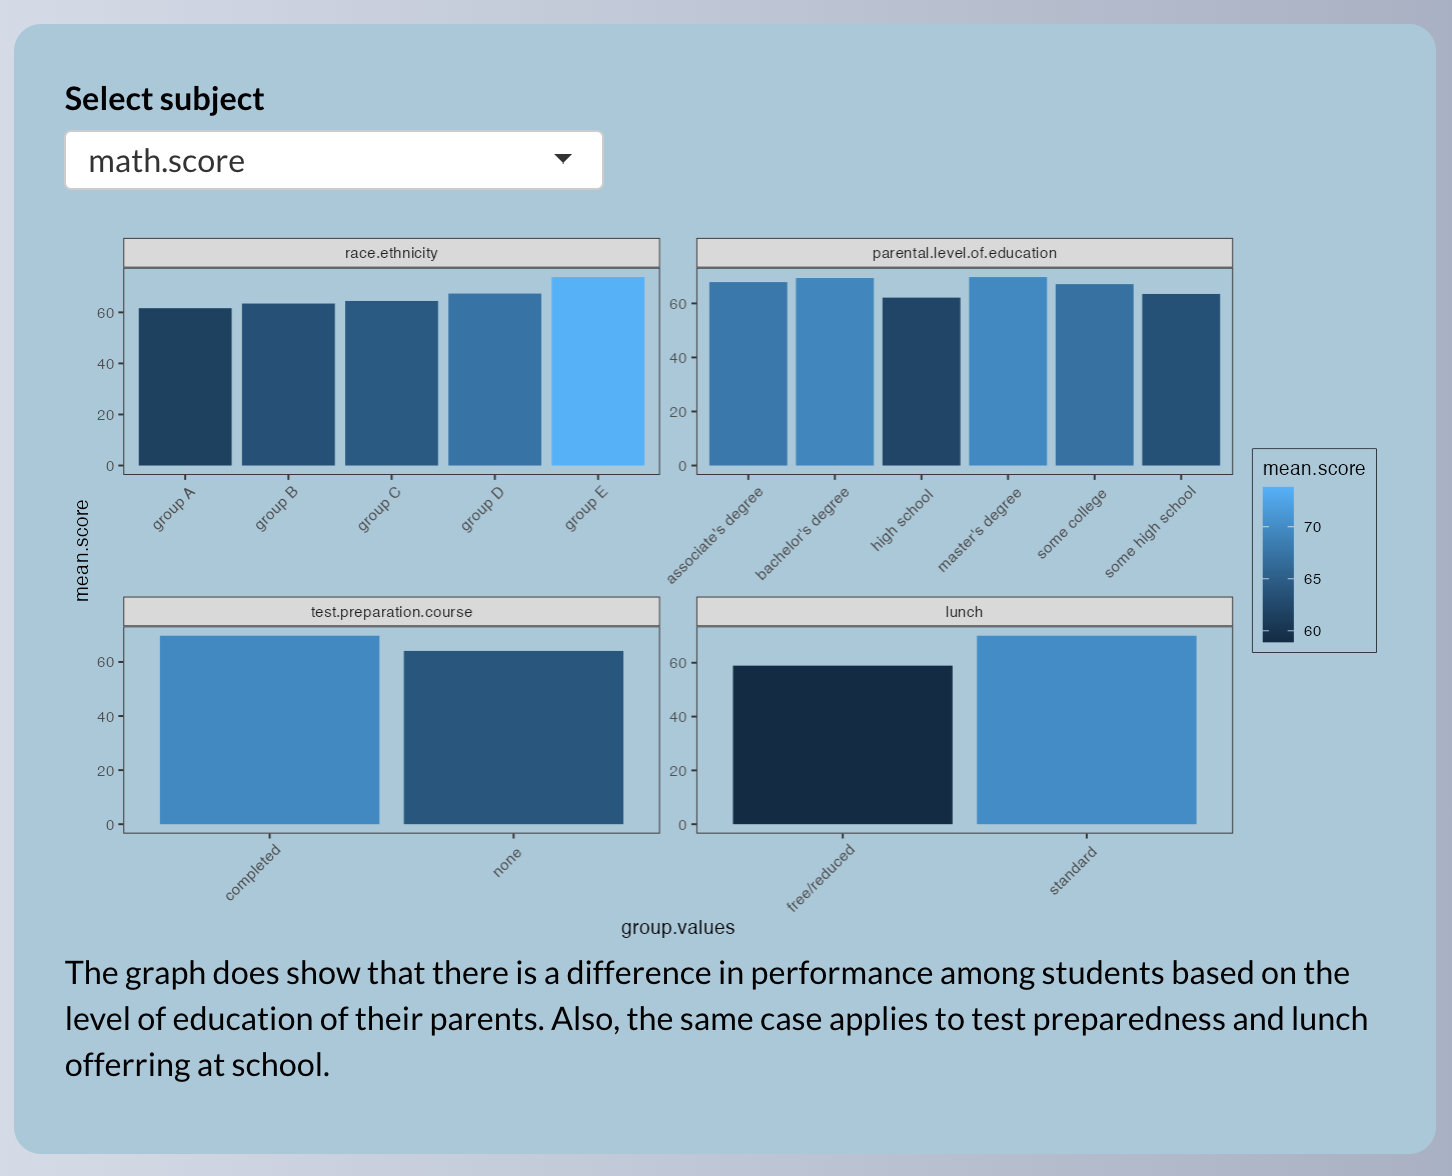
\includegraphics[width=5.20833in,height=2.08333in]{www/barcombined.png}

\newpage

\hypertarget{scatter-plot}{%
\subparagraph{Scatter plot}\label{scatter-plot}}

This is the go to graph whenever you want to see relationship between
two variables. In this case we used the scatter plot to show the
relationship between students performance in two subjects (math and
reading), further, we added a color aspect to the points to show the
gender comparisons. The relationship came out well, quite interesting to
see how the graph shows the differences in performance by gender for the
two subjects; boys performing well in math whereas the girls doing well
in reading.

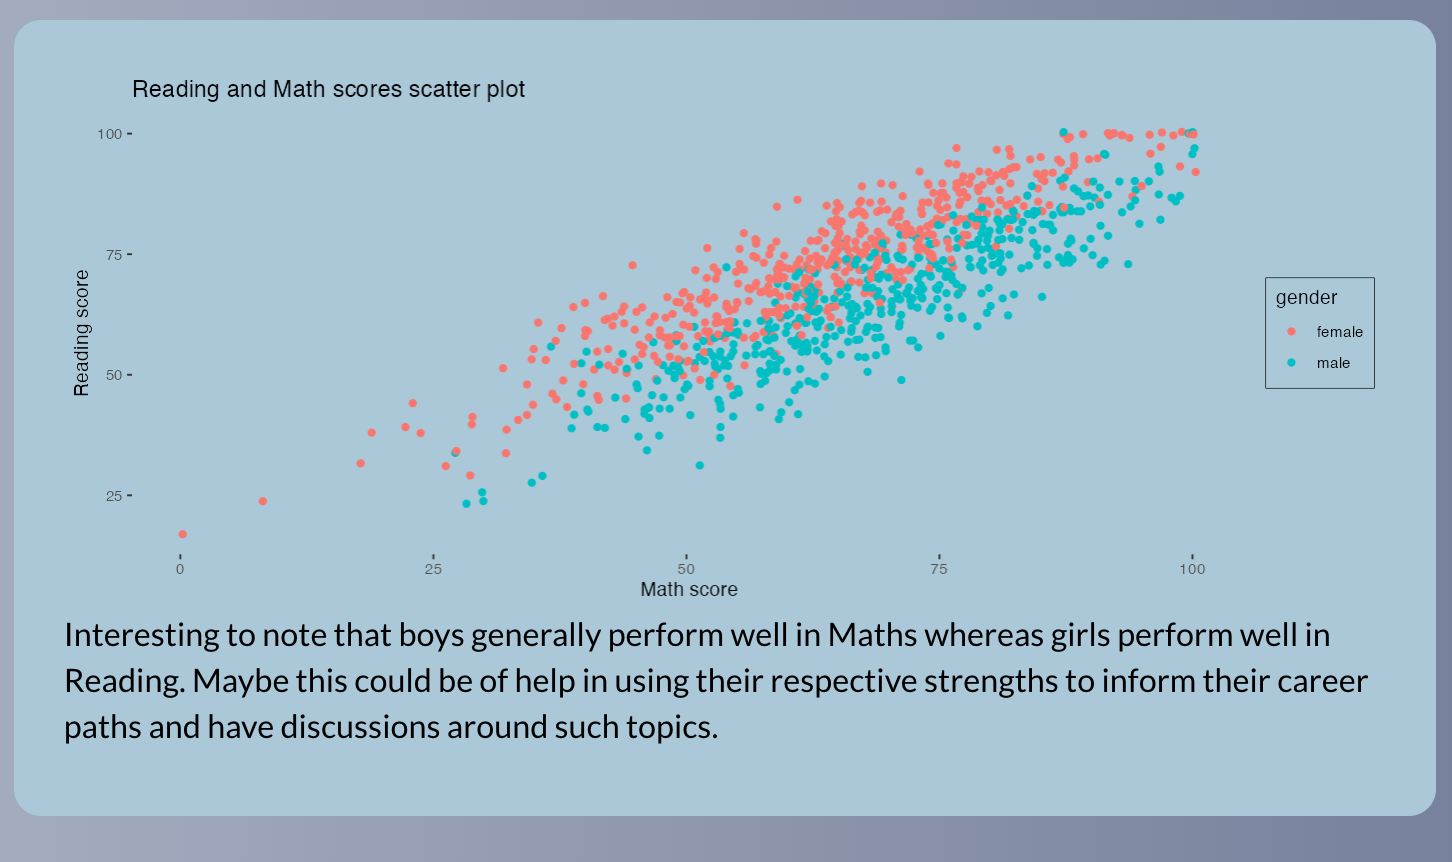
\includegraphics[width=5.20833in,height=2.08333in]{www/scatter.png}

\newpage

\hypertarget{grouped-bar-chart}{%
\subparagraph{Grouped bar chart}\label{grouped-bar-chart}}

The grouped bar chart is a good way to show comparison for the items of
a variable and how they compare in terms of quantities. This graph is
best for comparing quantities of categorical variable items. For this
case we use it show the average performance of boys and girls per
subject. Quite interesting to see how the graph show the gender
differences in performance across all subjects. Girls do well in reading
and writing whereas boys do well in math.

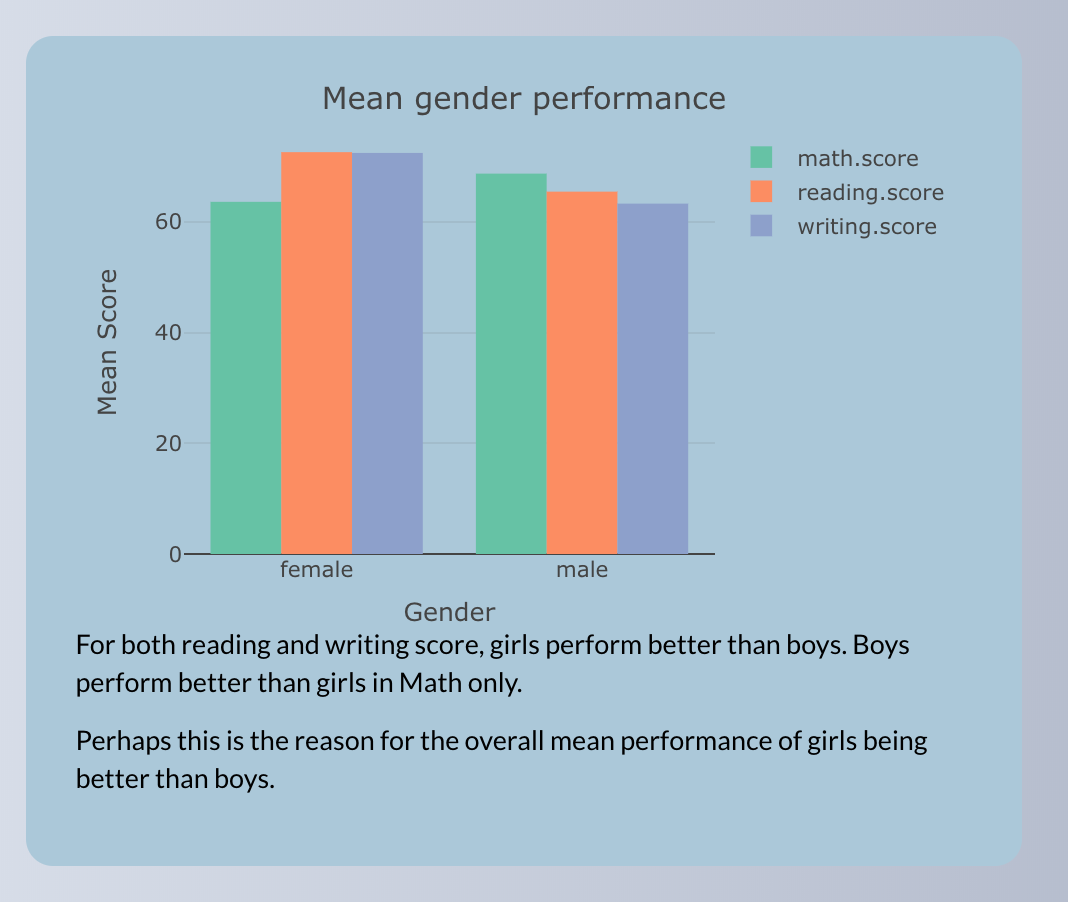
\includegraphics[width=5.20833in,height=2.08333in]{www/bar.png}

\newpage

\hypertarget{combined-bar-and-line-graph}{%
\subparagraph{Combined bar and line
graph}\label{combined-bar-and-line-graph}}

This is an amazing graph, being able to have two graphs on the same plot
with different scales. This helps to see the comparisons of variables
together as see how they relate if there be any kind of relationship.
For this case we have the line graph showing the number of students on
top of the bar graph that shows the student performance per ethnic
group. This graph has a dropdown menu that is used to select subjects
and have the graph show graph output for the selected subject.

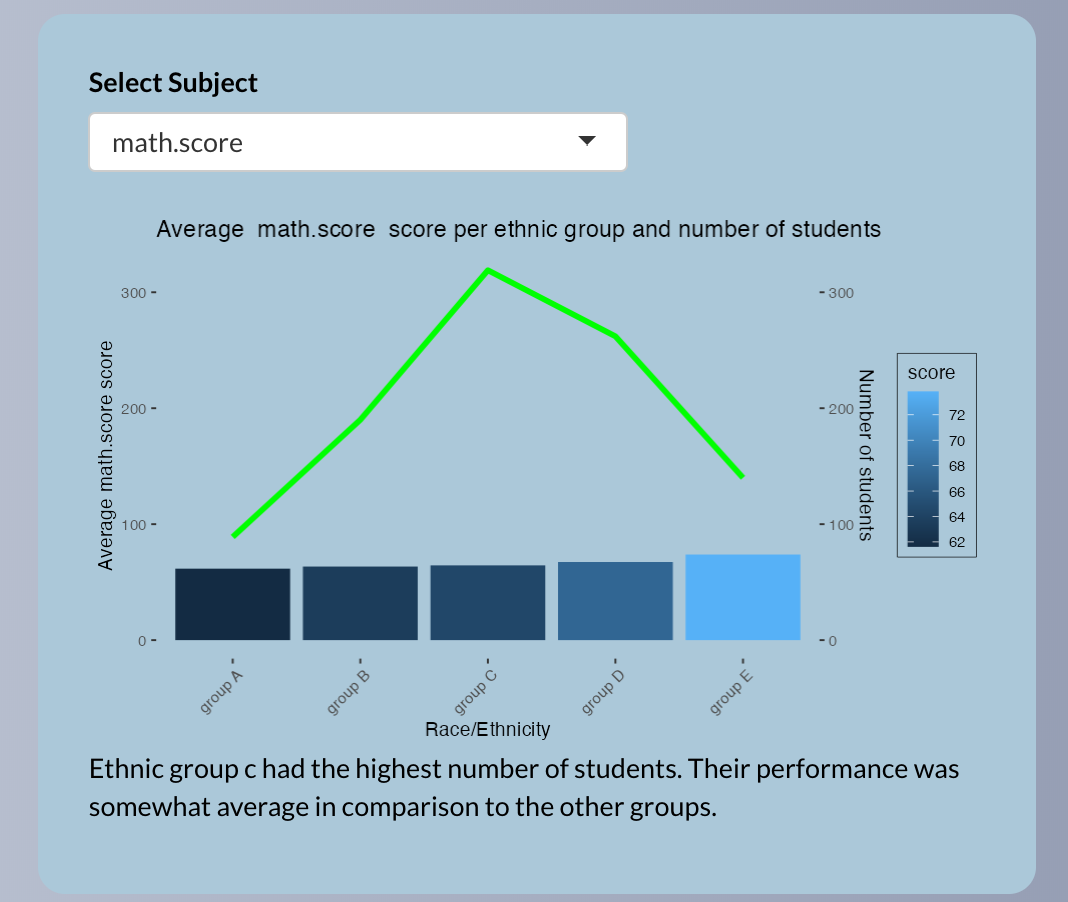
\includegraphics[width=5.20833in,height=2.08333in]{www/barlinegraph.png}

\hypertarget{heatmap}{%
\subparagraph{Heatmap}\label{heatmap}}

This is also a good alternative to scatter plot when you want to see
relationship between two variables. The data is presented in a two
dimensional panel whereby the color of the cell values shows the
magnitude in the values for the two variables in comparison. In this
case we want to see if there is any relationship between going out with
friends and number of hours spent studying in terms of performance.\\
There is a legend that shows the color intensity in relation to the
score values.

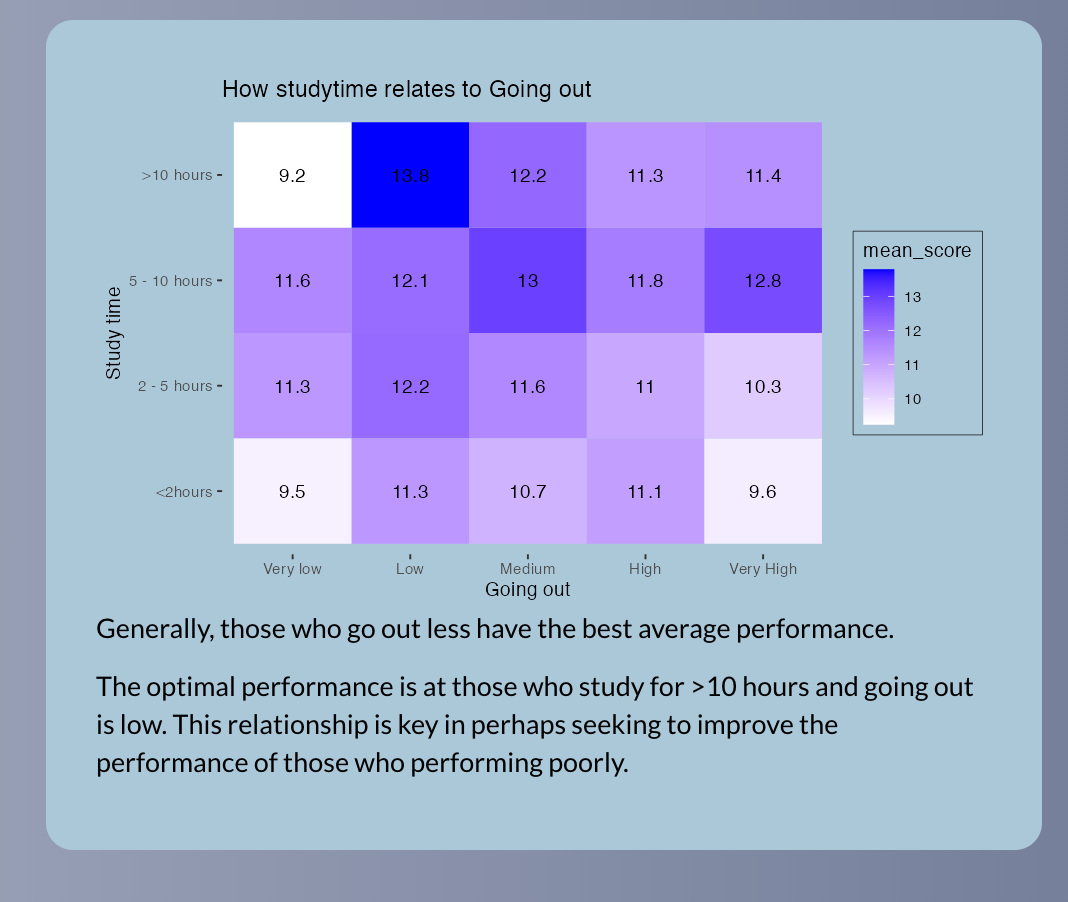
\includegraphics[width=5.20833in,height=2.08333in]{www/heatmap.png}

\hypertarget{conclusion-1}{%
\subsubsection{Conclusion}\label{conclusion-1}}

From the analysis of the various variables in the dataset, it is evident
that there are factors that contribute to the performance of students.\\
There are significant differences in student performance based on the
race/ethnicity, this might need further investigation as to why students
from certain races performed better than those from other ethnic
backgrounds.\\
The combination of the number of hours students spend studying and them
going out with friends revealed some sweet `spots' for optimal
performance, generally, the lower the going out the better the
performance, for the number of hours spent studying, the more the hours
the better the performance.

\hypertarget{references}{%
\paragraph{References}\label{references}}

\begin{enumerate}
\def\labelenumi{\arabic{enumi}.}
\item
  Alyahyan, E. D. (2020). Predicting academic success in higher
  education: Literature review and best practices. International Journal
  of Educational Technology in Higher Education, 17(1),
  \url{https://doi.org/10.1186/s41239-020-0177-7}
\item
  Cortez, P. (2008). Student Performance Data Set. UCI Machine Learning
  Repository: Student Performance Data Set. Retrieved April 23, 2023,
  from \url{https://archive.ics.uci.edu/ml/datasets/student+performance}
\item
  Seshapanpu, J. (2018). Students performance in exams. Kaggle.
  Retrieved April 23, 2023, from
  \url{https://www.kaggle.com/datasets/spscientist/students-performance-in-exams}
\end{enumerate}

\end{document}
